\chapter{PCN}
%http://portal.mec.gov.br/seb/arquivos/pdf/livro03.pdf
%Resumo http://www.somatematica.com.br/artigos/a3/
Os Parâmetros Curriculares Nacionais é umdocumento público que orienta aos professores como ministrarem aulas para os anos iniciais do Ensino Fundamental de forma a obter metas qualitativas determinadas.

''É importante destacar que a Matemática deverá ser vista pelo aluno como um conhecimento que pode favorecer o desenvolvimento do seu raciocínio, de sua sensibilidade expressiva, de sua sensibilidade estética e de sua imaginação'' (PCN's,1997)

\section{Alguns caminhos para “fazer Matemática” na sala de aula}

\subsection{Resolução de Problemas}

Existem vários bons motivos pelos quais aplicar a pespectiva de Resolução de Problemas como caminho para fazer Matemática em sala de aula. Um dos motivos é tal processo é utilizado como forma de avaliação por testes nacionais da qualidade da educação.  Por exemplo, a Provinha Brasil, que tem como objetivo avaliar a alfabetização das crianças matriculadas no $2^o$ ano de escolarização das escolas públicas. Como está escrito em \cite{da2011plano}, temos que ``as matrizes de referência que norteiam os testes de Matemática do Saeb e da Prova Brasil estão estruturadas sobre o foco Resolução de Problemas.''

Para os elaboradores desse teste a metodologia de Resolução de Problemas dá significado para o conhecimento matemático diante dos alunos enquanto esses têm situações desafiadoras para resolver e trabalham para desenvolver estratégias de resolução.

Ao colocar o foco na resolução de problemas, o que se defende é uma proposta que poderia
ser resumida nos seguintes princípios:

\begin{itemize}
    \item o ponto de partida da atividade matemática não é a definição, mas o problema. No processo de ensino e aprendizagem, conceitos, idéias e métodos matemáticos devem ser abordados mediante a exploração de problemas, ou seja, de situações em que os alunos precisem desenvolver algum tipo de estratégia para resolvê-las;
    \item o problema certamente não é um exercício em que o aluno aplica, de forma quase mecânica, uma fórmula ou um processo operatório. Só há problema se o aluno for levado a interpretar o enunciado da questão que lhe é posta e a estruturar a situação que lhe é apresentada;
    \item aproximações sucessivas ao conceito são construídas para resolver um certo tipo de problema; num outro momento, o aluno utiliza o que aprendeu para resolver outros, o que exige transferências, retificações, rupturas, segundo um processo análogo ao que se pode observar na história da Matemática;
    \item o aluno não constrói um conceito em resposta a um problema, mas constrói um campo de conceitos que tomam sentido num campo de problemas. Um conceito matemático se constrói articulado com outros conceitos, por meio de uma série de retificações e generalizações;
    \item a resolução de problemas não é uma atividade para ser desenvolvida em paralelo ou como aplicação da aprendizagem, mas uma orientação para a aprendizagem, pois proporciona o contexto em que se pode apreender conceitos, procedimentos e atitudes matemáticas.
\end{itemize}

Fica aqui recomendado a obra de Polya sobre a Resolução de Problemas em \cite{polya1995arte} que pode ser resumida nas duas páginas seguintes que podem ser encontradas no link  \url{http://www.miniweb.com.br/Ciencias/artigos/polya/Polya_Guzman.pdf}.
% ********** Ficha Catalográfica
%\newpage \normalsize
\thispagestyle{empty}

%\vspace{0.8cm}
\begin{footnotesize}
\begin{center}
\begin{tabular}{|cl|} \hline
\hspace{1cm} & \\
& Polya, G. (George), 1887- \\
P841a & \hspace{0.6cm}  A arte de resolver problemas: um novo aspecto do método matemático/G. Polya; \\ &tradução e adaptação Heitor Lisboa de Araújo. --2.reimp.--Rio de Janeiro: omtercoência, 1995.\\
& 196p.\\ \hline
\end{tabular}
\end{center}
\end{footnotesize}%\begin{small}
\hspace*{-1cm}

%https://pactuando.files.wordpress.com/2015/04/material-suporte-para-modulo-8-e-9-resoluu00c7u00c3o-de-problemas.pdf

%STANCANELLI, Renata. Conhecendo diferentes tipos de problemas. Ler, escrever e resolver problemas: habilidades básicas para aprender matemática. Porto Alegre: Artmed, p. 103-120, 2001.

%http://www.pead.faced.ufrgs.br/sites/publico/eixo4/matematica/espaco_forma/tipos_problemas/tipos_problemas.htm

\nocite{stancanelli2001conhecendo}

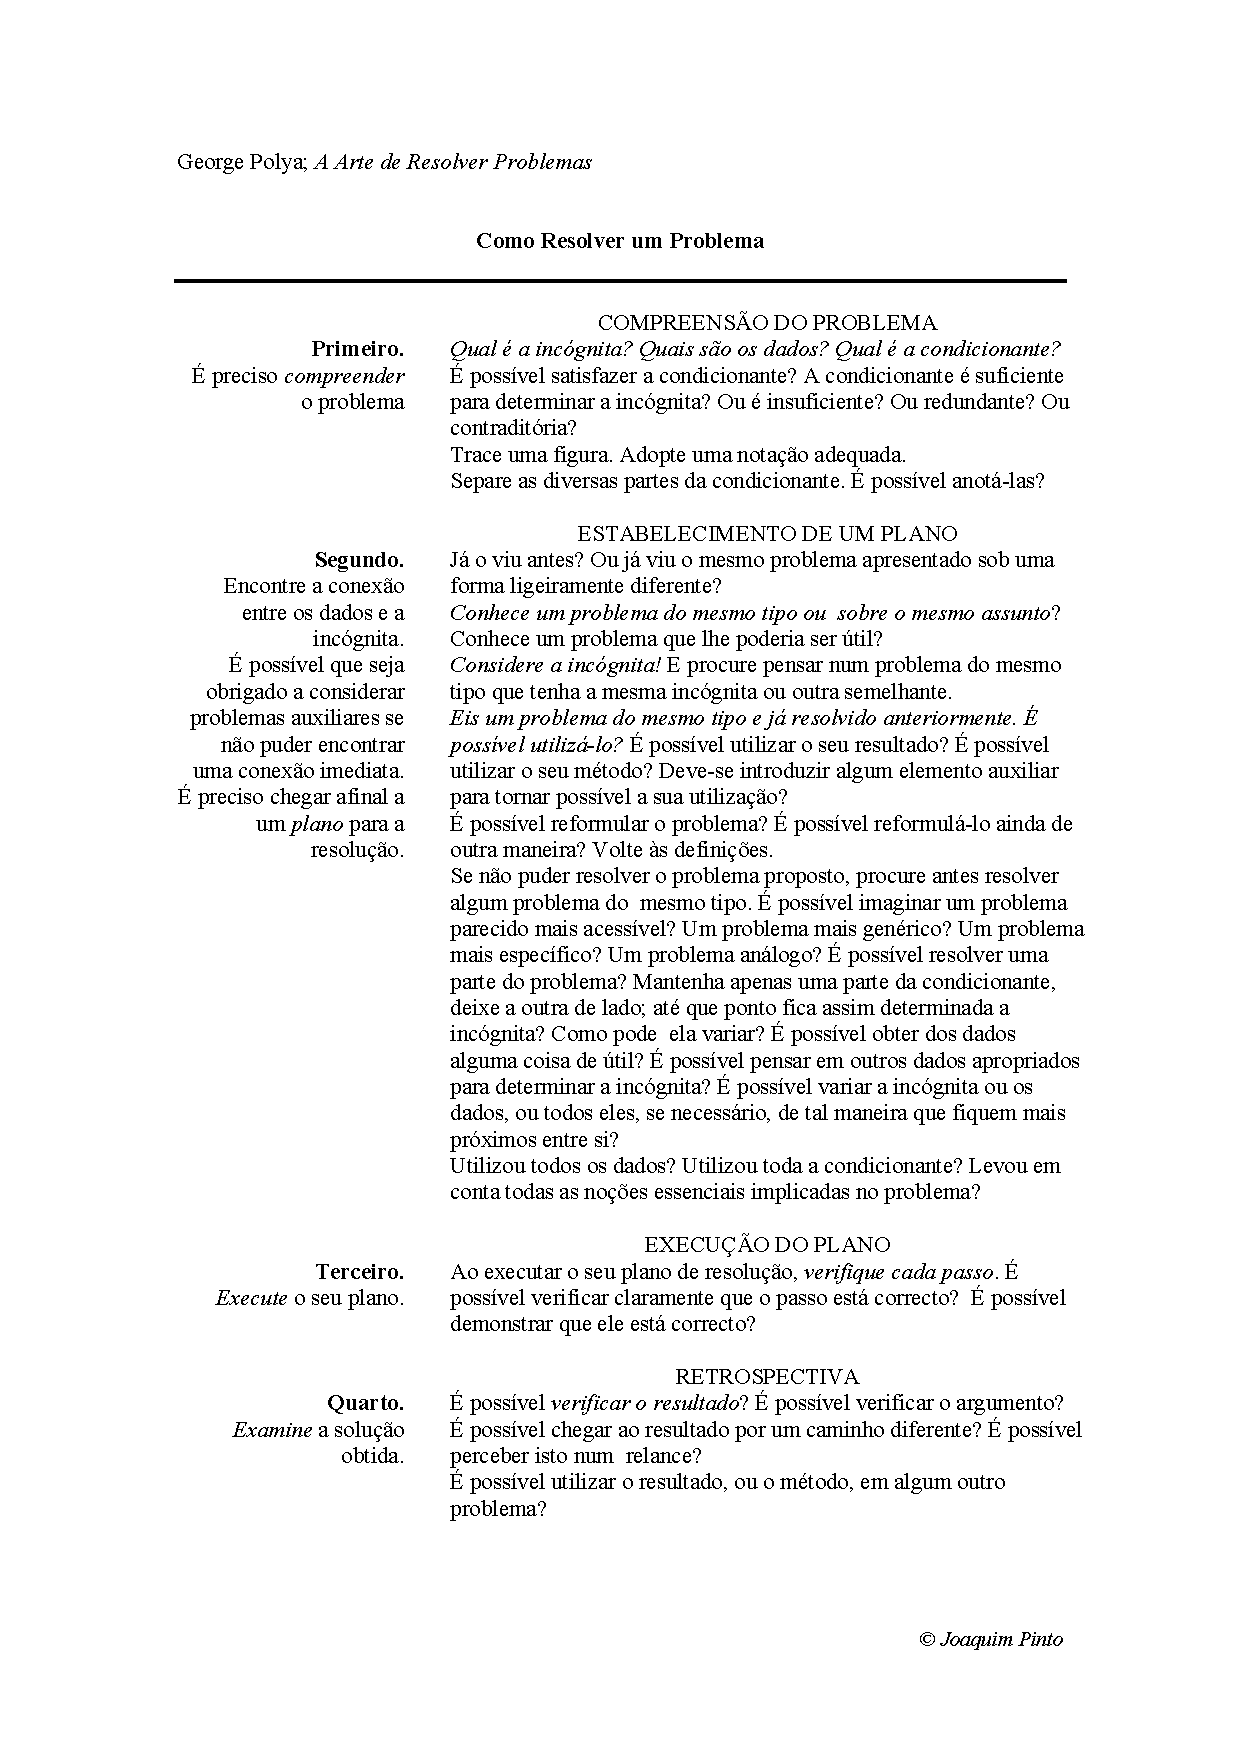
\includepdf[pages=-]{./part00/001.pdf}



\subsection{História da Matemática}

\nocite{roque2012historia}

\subsection{Tecnologias da Informação}

\subsection{Jogos}
http://www.fcc.org.br/pesquisa/publicacoes/cp/arquivos/613.pdf

\section{Objetivos da Matemática para o Ensino Fundamental}

\begin{enumerate}
    \item identificar os conhecimentos matemáticos como meios para compreender e \textbf{transformar o mundo à sua volta} e perceber o caráter de jogo intelectual, característico da Matemática, como aspecto que estimula o interesse, a curiosidade, o espírito de investigação e o \textbf{desenvolvimento da capacidade para resolver problemas};
    
    \item fazer observações sistemáticas de \textbf{aspectos quantitativos e qualitativos} do ponto de vista do conhecimento e estabelecer o maior número possível de relações entre eles, utilizando para isso o conhecimento matemático (aritmético, geométrico, métrico, algébrico, estatístico, combinatório, probabilístico); selecionar, organizar e \textbf{produzir informações relevantes, para interpretá-las e avaliá-las criticamente};
    
    \item resolver situações-problema, sabendo validar estratégias e resultados, desenvolvendo formas de raciocínio e processos, como \textbf{dedução, indução, intuição, analogia, estimativa}, e utilizando conceitos e procedimentos matemáticos, bem como instrumentos tecnológicos disponíveis;
    
    \item comunicar-se matematicamente, ou seja, descrever, representar e apresentar resultados com precisão e argumentar sobre suas conjecturas, fazendo uso da linguagem oral e estabelecendo relações entre ela e diferentes representações matemáticas;
    
    \item estabelecer conexões entre temas matemáticos de diferentes campos e entre esses temas e conhecimentos de outras áreas curriculares;
    
    \item sentir-se seguro da própria capacidade de construir conhecimentos matemáticos, desenvolvendo a auto-estima e a perseverança na busca de soluções;
    
    \item interagir com seus pares de forma cooperativa, trabalhando coletivamente na busca de soluções para problemas propostos, identificando aspectos consensuais ou não na discussão de um assunto, respeitando o modo de pensar dos colegas e aprendendo com eles.
\end{enumerate}

\section{Bloco de Conteúdos}

\subsection{Números e Operações}

Ao longo do ensino fundamental os conhecimentos numéricos são construídos e assimilados pelos alunos num \textbf{processo dialético}, em que intervêm como instrumentos eficazes para resolver determinados problemas e como objetos que serão estudados, considerando-se suas \textbf{propriedades, relações e o modo como se configuram historicamente}.
 
Nesse processo, o aluno perceberá a existência de diversas \textbf{categorias numéricas criadas em função de diferentes problemas que a humanidade teve que enfrentar} — números naturais, números inteiros positivos e negativos, números racionais (com representações fracionárias e decimais) e números irracionais. À medida que se deparar com\textbf{ situações-problema — envolvendo adição, subtração, multiplicação, divisão, potenciação e radiciação —, ele irá ampliando seu conceito de número}.

Com relação às \textbf{operações}, o trabalho a ser realizado se concentrará na \textbf{compreensão dos diferentes significados de cada uma delas}, nas \textbf{relações existentes entre elas} e no \textbf{estudo reflexivo do cálculo}, contemplando diferentes tipos — \textbf{exato e aproximado},\textbf{ mental e escrito}. Embora nas séries iniciais já se possa desenvolver uma pré-álgebra, é especialmente nas séries finais do ensino fundamental que os trabalhos algébricos serão ampliados; trabalhando com situações-problema, o aluno \textbf{reconhecerá diferentes funções da álgebra} (\textbf{como modelizar, resolver problemas aritmeticamente insolúveis, demonstrar}), representando problemas por meio de equações (identificando parâmetros, variáveis e relações e tomando contato com fórmulas, equações, variáveis e incógnitas) e conhecendo a “sintaxe” (regras para resolução) de uma equação.


\subsection{Espaço e Forma}

\subsection{Grandezas e Medidas}

\subsection{Tratamento da Informação}

\section{Conteúdos atitudinais do primeiro e segundo cíclo}

\subsection{Primeiro cíclo}

\subsection{Segundo cíclo}

\section{Descritores. O que são e para que servem?}
%http://portal.inep.gov.br/web/saeb/32
%http://www.pucrs.br/edipucrs/erematsul/comunicacoes/17ISABELCRISTINA.pdf

Os descritores da Prova Brasil foram criados baseados nas propostas curriculares de alguns estados e municípios e os PCNs. O MEC então fês uma matriz de referência baseada nelas.

%Complementos de Matemática para professores do Ensino Básico

\subsection{Explorando a soma nos naturais}
%\footnote{\href{http://portal.mec.gov.br/seb/arquivos/pdf/livro03.pdf}{Parâmetros Curriculares Nacionais}}
Os PCNs oriemtam que a soma sejam trabalhados de algumas formas específicas. Temos por exemplo que a adição deve ser trabalhada em conjunto com a subtração. 
São elencado quatros principais grupos de ideias relacionadasa soma:

\subsubsection{Combinar/Juntar}

Exemplo:

Em uma classe há 15 meninos e 13 meninas. Quantas crianças há nessa classe?

A partir dessa situação é possível formular outras duas, mudando-se a pergunta. As novas situações são comumente identificadas como ações de \textbf{“separar/tirar”}. Exemplos:

— Em uma classe há alguns meninos e 13 meninas, no total são 28 alunos. Quantos menino há nessa classe?

— Em uma classe de 28 alunos, 15 são meninos. Quantas são as meninas?

\subsubsection{Transformação}

Num segundo grupo, estão as situações ligadas à idéia de transformação, ou seja, alteração de um estado inicial, que pode ser positiva ou negativa. Exemplos:

— Paulo tinha 20 figurinhas. Ele ganhou 15 figurinhas num jogo. Quantas figurinhas ele tem agora? (transformação positiva).

— Pedro tinha 37 figurinhas. Ele perdeu 12 num jogo. Quantas figurinhas ele tem agora? (transformação negativa).

Cada uma dessas situações pode gerar outras:

— Paulo tinha algumas figurinhas, ganhou 12 no jogo e ficou com 20. Quantas figurinhas ele possuía?

— Paulo tinha 20 figurinhas, ganhou algumas e ficou com 27. Quantas figurinhas ele ganhou?

— No início de um jogo, Pedro tinha algumas figurinhas. No decorrer do jogo ele perdeu e terminou o jogo com 7 figurinhas. Quantas figurinhas ele possuía no início do jogo?

— No início de um jogo Pedro tinha 20 figurinhas. Ele terminou o jogo com 8 figurinhas. O que aconteceu no decorrer do jogo?

\subsubsection{Comparação}
Num terceiro grupo, estão as situações ligadas à idéia de comparação.
Exemplo:

— No final de um jogo, Paulo e Carlos conferiram suas figurinhas. Paulo tinha 20 e Carlos tinha 10 a mais que Paulo. Quantas eram as figurinhas de Carlos?

Se se alterar a formulação do problema e a proposição da pergunta, incorporando ora dados positivos, ora dados negativos, podem-se gerar várias outras situações:

— Paulo e Carlos conferiram suas figurinhas. Paulo tem 12 e Carlos, 7. Quantas figurinhas Carlos deve ganhar para ter o mesmo número que Paulo?
— Paulo tem 20 figurinhas. Carlos tem 7 figurinhas a menos que Paulo. Quantas figurinhas tem Carlos? 71

\subsubsection{Composição de transformações}
Num quarto grupo, estão as situações que supõem a compreensão de mais de uma transformação (positiva ou negativa). Exemplo:

— No início de uma partida, Ricardo tinha um certo número de pontos. No decorrer do jogo ele ganhou 10 pontos e, em seguida, ganhou 25 pontos. O que aconteceu com seus pontos no final do jogo?

Também neste caso as variações positivas e negativas podem levar a novas situações:

— No início de uma partida, Ricardo tinha um certo número de pontos. No decorrer do jogo ele perdeu 20 pontos e ganhou 7 pontos. O que aconteceu com seus pontos no final do jogo?

— Ricardo iniciou uma partida com 15 pontos de desvantagem. Ele terminou o jogo com 30 pontos de vantagem. O que aconteceu durante o jogo?

Embora todas estas situações façam parte do campo aditivo, elas colocam em evidência níveis diferentes de complexidade. Note-se que no início da aprendizagem escolar os alunos ainda não dispõem de conhecimentos e competências para resolver todas elas, necessitando de uma ampla experiência com situações-problema que os leve a desenvolver raciocínios mais complexos por meio de tentativas, explorações e reflexões.

Desse modo, o trabalho com as operações deve ser planejado coletivamente pelos professores, não apenas para ser desenvolvido nos dois primeiros ciclos, mas também na quinta e sexta séries.

\section{Números Racionais}

Nos PCN \cite{brasil2008pde} o conjunto dos números racionais surge como um subtema da grande área de Números e Operações. Na seção de Organização dos Conteúdos é dito que um tema deve ser abordado visando as conecções com outros conteúdos, foco nos pontos mais fundamentais e o nível da profundidade em que será trabalhado em cada um de seus ciclos.

Os números racionais tem diversas interconecções com muitos conteúdos, mas só recebem destaque durante o segundo ciclo do Ensino Fundamental e se estabelece sobre conceitos que se estruturaram no ciclo anterior, já que

\begin{quote}
Neste ciclo, são apresentadas aos alunos situações-problema cujas soluções não se encontram no campo dos números naturais, possibilitando, assim, que eles se aproximem da noção de número racional. \cite{brasil2008pde}
\end{quote}

É dito que os alunos devem construir o significado do número racional e de suas representações (fracionária e decimal), a partir de seus diferentes usos no contexto social. Porém vemos que o foco se encontra na sua forma decimal devido à disseminação das calculadoras e de outros instrumentos
que a utilizam.

\section{Teoria dos Conjuntos}

A assim chamada ``Teoria dos Conjuntos'' era apenas a ponta emergente de uma visão estruturalista mais vasta, de inspiração boubakista, da Matemática, que teve várias denominações: Nova Matemática, Matemática moderna e outras mais.\cite{d2007elementos}